The Gross-Pitaeskii equation is the Hatree model.  So does the Bogolubov approach, they are just the assumption of the BEC form for the many-body equation.  The close-channel molecule is in some way bosons, which is not affected by Pauli-principle.  We have to go one-level deeper to take the Pauli-principle in.   That is kind of related to the two-fermion-composite-molecule gas, and the cobosons idea.  But I am not sure whether ideas there \cite{CobosonPhysicsReports,CobosonCalculation} help. 


So for the dilute coboson gas, the question is that how does the two-body correlation, which is the same as two-body molecule solution in the lowest order, affected by the many-body nature.  In the normal language, only the center of mass coordinator is considered. We are more interested in the opposite side, how does the relatively coordinator changes? In terms of real-space, probably only long-scale is modified.  But in terms of the momentum-space, a molecule has much more spread momentum, with no way to define things like Fermi surface.  How does Pauli-principle work here?

\subsection{Talk with Gordon}
He pointed out that I am looking for is as such, open->close<->open. And he mentioned Petrov's work. \cite{Petrov}  That is also looking into two cobosons, but that is not exactly what I am looking forward.  See figure \ref{fig:openClose}.
\begin{figure}[htb]
	\centering
		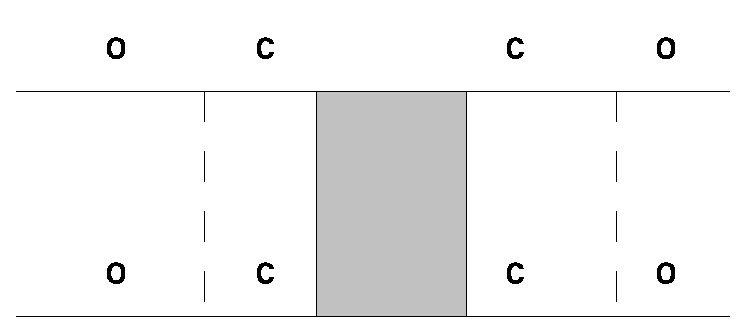
\includegraphics[width=.50\textwidth]{image/openClose.eps}
	\caption{Open-Close Interaction\label{fig:openClose}}
	
\end{figure}

\subsection{}
In the perturbation suggested by Tony, the nature how close-channel molucule involved in the many-body is also needed.  So either way, how two-fermion cobosons gas evolves are important.  Pertrov \cite{Petrov} gives $0.6a_s$ for two molecules interacted.  But does not give the information about how the w.f. changes, which is probably more interested for my problem as this afftects the open-channel component.  Furthermore, he does not specify how the many-body set in. 
So the first thing to do is to find out how many-body change the close-channel.   
